\section{Methods I: Kinemetry analysis}
\label{sec:methods-I-kinemetry}

\subsection{Kinemetry analysis method description}
\label{kinemetry-analysis-method-description}
% \subsection{Quality screening}
Global kinematic velocity position angles (PA) for the PSB and control galaxy samples were determined using the \texttt{fit\_kinemetry\_pa} routine as described in appendix C of \cite{2006MNRAS.366..787K}. The routine returns the angle of the line bisecting the greatest change in velocity between the receding and approaching sides. \cite{2019MNRAS.483..172D} performed a \texttt{kinemetry} analysis of over 8,000 galaxies from the internal MPL-8 release of the MaNGA survey. In order to obtain a clean sample of well defined global PAs they visually classified the stellar and H$\alpha$ gas velocity fields of all galaxies in their sample into 3 categories (Chris Duckworth, 2019, personal communication), and set flags in their dataset as follows:

\begin{itemize}
    \item {Flag 1} : Dominant coherent rotation and well defined PA. 
    \item {Flag 2} : Dominant coherent rotation but with complex motions or highly inclined velocity fields 
    \item {Flag 3} : Do not use
\end{itemize}

During this analysis galaxies with kinematically decoupled cores (KDCs) and warped velocity fields were also identified.

The resulting MPL-8 screened dataset from dataset of galaxies with reliable global PAs (flagged as [1] or [2]) from \cite{2019MNRAS.483..172D} was matched with the PSB galaxies in the sample of Chen et al. (2019, in prep.) to obtain a subset of PSBs with good \texttt{kinemetry} analysis flags. Furthermore a subset of those PSBs with $\Delta$PAs > 30\textdegree\ was extracted. The results are shown in Tables \ref{tab:my-CPSBs} and \ref{tab:my-RPSBs}. 

An example of galaxies with aligned and misaligned stellar an gas velocity fields is shown in Figure \ref{} 

In classical Kinemetry analysis it is considered significant if the $\Delta$PA position angle is greater than 30 degrees. We show some examples of misaligned stellar and gas velocity fields here: 
[TODO: tidy up this section.]

\begin{figure}[h]
    \centering
    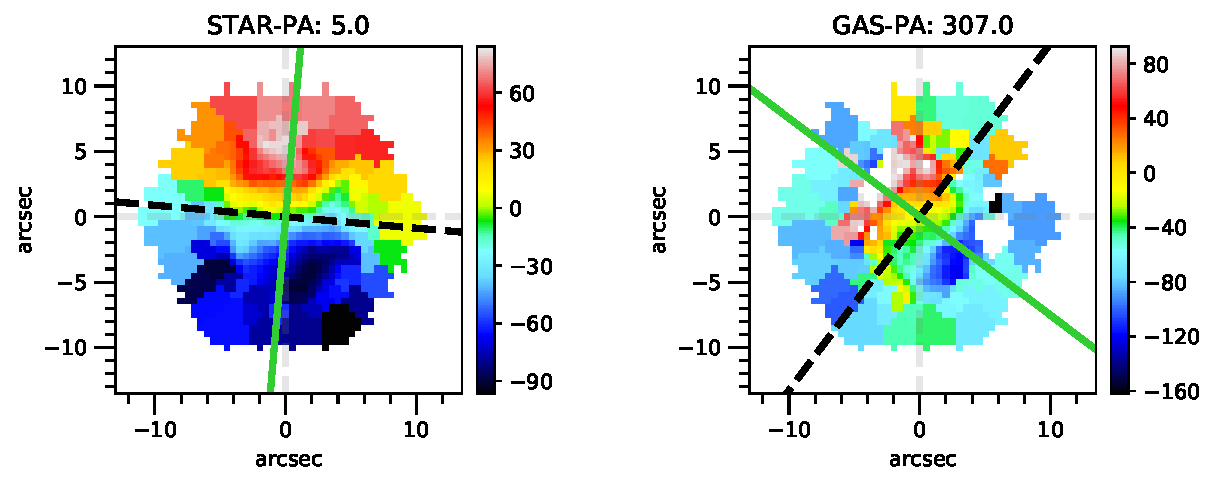
\includegraphics[width=\columnwidth]{images/PAplots/PAplotsCPSB/8313-6101-PA.pdf}
    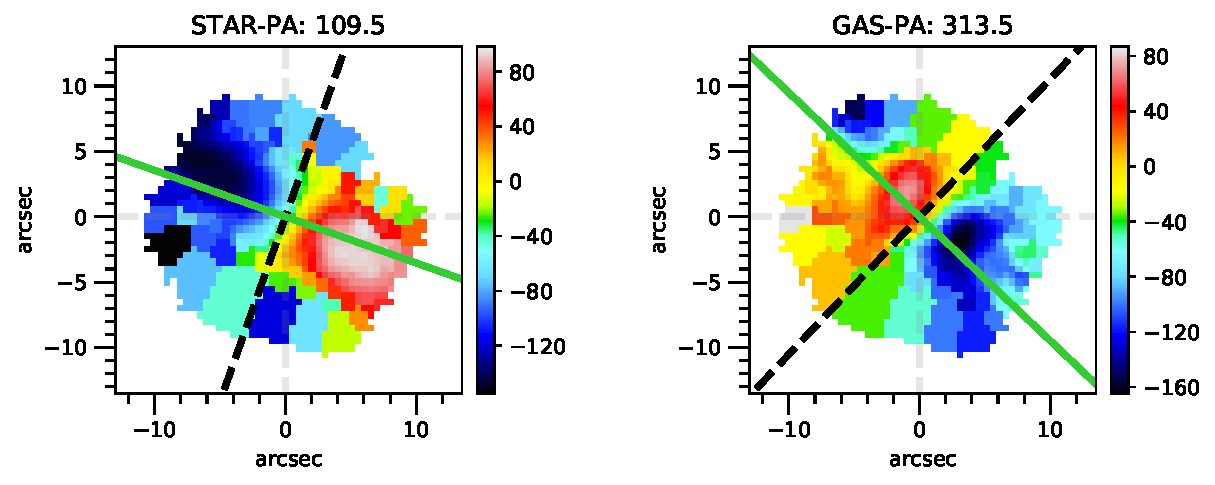
\includegraphics[width=\columnwidth]{images/PAplots/PAplotsRPSB/8323-6103-PA.pdf}
    \caption{Kinemetry-derived position angles (PA) for stellar velocity (left) and gas velocity (right) of two PSB galaxies exhibiting a significant $\Delta$PA. Top: CPSB 8313-6101, and bottom: RPSB 8323-6103. The velocity position angle is displayed as the green solid line while the black dashed line denotes the bisector of the velocity field between the receding (red) and blue (approaching) sides. The velocity colour scale is \kms. Credit for data analysis and plots: Chris Duckworth.}
    \label{fig:CPSB-8313-6101-PA}
\end{figure}

\subsection{Position angle misalignment}
\label{PA-misalignment}
The results of the gas and velocity field position angle misalignment measurements for PSBs where the $\Delta$PA \textgreater 30\textdegree are tabulated in Figure \ref{tab:offsetCPSBs} for the CPSBs, and Figure \ref{tab:offsetRPSBs} for the RPSBs. 

\begin{table}[h]
\centering
\caption{CPSBs with gas and stellar velocity kinematic PA offsets \textgreater 30\textdegree.}
\label{tab:offsetCPSBs}
\begin{tabular}{lccc}
\hline
PlateIFU  & Stellar PA & H$\alpha$ PA & $\Delta$PA \\
  & (deg.) & (deg.) & (deg.) \\
\hline
8313-6101 & 5 & 307 & 58 \\
8655-1902 & 335 & 127 & 152 \\
8725-1902 & 22 & 175 & 153 \\
8938-6102 & 214 & 47.5 & 166.5 \\
9494-3701 & 140.5 & 243 & 102.5 \\
\hline
\end{tabular}
\end{table}

\begin{table}[h]
\centering
\caption{RPSBs with gas and stellar velocity kinematic PA offsets \textgreater 30 \textdegree.}
\label{tab:offsetRPSBs}
\begin{tabular}{lccc}
\hline
PlateIFU   & Stellar PA & H$\alpha$ PA & $\Delta$PA \\
  & (deg.) & (deg.) & (deg.) \\
\hline
8080-3704 & 24 & 154 & 130 \\
8262-3701 & 153.5 & 118.5 & 35 \\
8323-6103 & 109.5 & 313.5 & 156 \\
8439-6104 & 5.5 & 107 & 101.5 \\
8453-3704 & 44 & 91 & 47 \\
8486-1901 & 295.5 & 85 & 149.5 \\
8554-3701 & 250 & 68 & 178 \\
8932-12704 & 166.5 & 134.5 & 32 \\
9872-3701 & 208.5 & 81 & 127.5 \\
\hline
\end{tabular}
\end{table}

The number of PSBs with galaxies clearly defined $\Delta$PAs is small fraction of the sample: 5 out of 30 CPSBs, and 9 out of 37 RPSBs. It can be noted that RPSBs possess extensive star forming regions while CPSBs generally do not. RPSBs should therefore have comparatively more gas than CPSBs.
